\chapter{Czech datasets}
Despite the relatively satisfying number of datasets, there is essentially no Czech dataset which is at 
\section{Translation}
\subsection{DeepL}
\section{Processing}
\section{Analysis}
output \= unified set of Czech bias related datasets
\textbf{Czech Unified set of Bias Data}
\begin{enumerate}
    \item mpqa-cs
    \item subj-cs
    \item newsb-cs
    \item cw-hard-cs
    \item wiki-npov-large-cs
    \item babe-cs
\end{enumerate}

\newpage

\section{Czech Wiki neutrality corpus}
Finally, I present two novel parallel corpora extracted directly from Czech Wikipedia. To my best knowledge, this is the only original Czech dataset related to media bias or subjectivity detection.
I followed two main approaches of extraction of the sentences, both of them relying on the extraction of revisions that includes the \{\{NPOV\}\} tag or its variation. The NPOV tag has also its Czech version \Gls{nup}. However, the czech version is practically not used and so for the extraction, the english variations were used.

\subsubsection{WIKI1-CS}
For this dataset I followed the \cite{aleksandrova2019multilingual} approach and their script. First, a file with all pages and its complete edit history is downloaded from wiki dump. I used the "20220201" version. Then the edits containing one of the NPOV related tags are extracted and then the process of sentence extraction follows.
This approach yielded 15k sentences, However, it uses rather trivial assumption that when NPOV tag is removed, all removed sentences are extracted as biased and all added are introduced as unbiased. This annotating strategy later [odkaz na experimenty] proved to be insuffiecient and yielded very noisy dataset.

\subsubsection{WIKI2-CS}
This dataset was created following \cite{pryzant2020automatically} approach. Here the process is the same as described in section \ref{wiki}. I used "20210920" snapshot of wikipedia and slighlty modified authors script to fit the czech language properties. Namely regex alternation and czech tokenizer. This resulted in
\begin{enumerate}
    \item 3k of "before" and "after" sentence pairs
    \item 1.7k subset of mentioned set where only one word was changed
    \item 7.5 sentences, where the change was rejected or reversed implying neutrality of the original sentence
    
The random example of sentence pair can be seen in \ref{fig:wiki2cs-example}

\newpage
\begin{figure}
  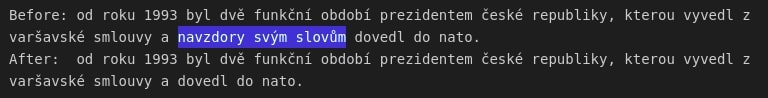
\includegraphics[width=\linewidth]{my_modules/multimedia/wiki2example.jpg}
  \caption{Example of sentence pair}
  \label{fig:wiki2cs-example}
\end{figure}

\end{enumerate}
